\section{Neuronale Netze}
\label{sec:neuralnet}
In diesem Kapitel werden wir eine weitere Möglichkeit betrachen, ein Anfangswertproblem zu lösen.
Dabei gehen wir genauer auf neuronale Netze ein. Dieser Abschnitt bezieht sich hauptsächlich auf
\cite{ovidiucalinDeepLearningArchitectures}. Obwohl die bisher besprochenen numerischen Verfahen wie Runge-Kutta- und
Mehrschrittverfahren heutzutage extrem effizient in Bezug auf Fehlertoleranz und Rechenaufwand sind, gibt es dennoch
Vorteile neuronale Netze zu benutzen. Falls Beispielsweise die Interesse besteht, die Lösung einer gewöhnlichen
Differentialgleichung nur in einem bestimmten Zeitpunkt $\hat{t}$ auszuwerten, so müssen in numerischen Verfahren von
der Anfangszeit $t_0$ bis zur gewünschten Zeit $\hat{t}$ iteriert werden. Ein \textit{trainiertes} neuronales Netz
repräsentiert jedoch die gesuchte Lösung und ist deshalb in der Lage eine Funktionsauswertung in $\hat{t}$ auszuführen,
was im Gegensatz zu den numerischen Verfahren viel Rechenarbeit spart. Neuronale Netze haben in Bezug auf das
Approximieren mehrerer Differentialgleichungen noch einen ausschlaggebenden Vorteil für die Recheneffizienz, welchen
wir in Abschnitt \ref{subsec:lsgpakete}betrachten werden.

\subsection{Struktur neuronaler Netze}
\label{subsec:struktur-eines-neuronalen-netzes}
Zur Übersicht beschränken wir uns zuerst auf ein neuronales Netz mit einer Eingangsschicht mit $3$ Neuronen, zwei
versteckte Schichten mit jeweils 3 Neuronen und eine Ausgangsschicht mit 2 Neuronen wie in Abbildung
\eqref{neuralNetexample} dargestellt. Die gelben Neuronen repräsentieren hier jeweils ein \textit{on-Neuron}, oder
\textit{bias}, welches konstant $x_0^{(l)} = -1$ ist. Allgemein haben wir $L$ Schichten und $n^{(l)}$, $l=1, \dots, L$,
Neuronen pro Schicht, wobei der bias ausgeschlossen ist. Die Gewichte $\omega_{ij}^{l}$ geben an, in welcher Relation
die Neuronen der vorherigen Schicht $l-1$ zu den Neuronen der nächsten Schicht $l$ stehen. Dabei werden die Gewichte
der Bias-Neuronen mit $b_j^{(l)}:= \omega_{0j}^{(l)}$ von den anderen Gewichten unterschieden.
\begin{figure}[htp]
    \centering
    \begin{neuralnetwork}[height=4]
        \newcommand{\x}[2]{$x^{(0)}_#2$}
        \newcommand{\y}[2]{$y_#2$}
        \newcommand{\hfirst}[2]{\small $x^{(1)}_#2$}
        \newcommand{\hsecond}[2]{\small $x^{(2)}_#2$}
        \inputlayer[count=3, bias=true, title=Eingabe-\\schicht, text=\x]
        \hiddenlayer[count=3, bias=true, title=versteckte\\Schicht 1, text=\hfirst]
        \linklayers
        \hiddenlayer[count=3, bias=true, title=versteckte\\Schicht 2, text=\hsecond]
        \linklayers
        \outputlayer[count=2, title=Ausgabe-\\schicht, text=\y] \linklayers
    \end{neuralnetwork}
    \caption{neuronales Netzwerk mit 3 Eingabeneuronen (grün), bias (gelb), zwei versteckte Schichten
        (blau) und 2 Ausgabeneuronen (rot)}
    \label{neuralNetexample}
\end{figure}
Die Signale der Neuronen ab der ersten versteckten Schicht bilden sich aus der Summe aller vorherigen
Signale mit entsprechender Gewichtung:
\begin{align}
    s_j^{(l)} = \sum_{i=1}^{n^{(l)}} \omega_{ij}^{(l)} x_i^{(l-1)} - b_j^{(l)}. \label{eq:signal}
\end{align}
Darauffolgend ergeben sich die Ausgaben der nächsten Schicht $l$
\begin{align}
    x_j^{(l)}=\Psi(s_j^{(l)}). \label{eq:activ}
\end{align}
Dabei ist $\Psi: \mathbb{R} \rightarrow \mathbb{R}$ die sogenannte \textit{Aktivierungsfunktion}. In unserer Anwendung
werden wir hauptsächlich den \textit{Tangens hyperbolicus}
\[
    \tanh(x)=\frac{e^x - e^{-x}}{e^x + e^{-x}}
\]
als Aktivierungsfunktion nutzen. Das Trainieren eines neuronalen Netzes lässt sich im Grunde auf ein Minimierungsproblem
einer \textit{Kostenfunktion} $\mathcal{C}$
%\[
%    \mathcal{C}: \mathbb{R}^{\left(n^{(l-1)} + 1\right) \times n^{(l)} \times L} \rightarrow \mathbb{R}
%\]
reduzieren. Dazu werden die Konzepte der Forward- und Backwardpropagation, sowie ein \textit{Gradientenverfahren}
benötigt, was wir in den folgenden Teilabschnitten besprechen werden.

\subsubsection{Forwardpropagation}
{\em Forward propagation} wird der Vorgang genannt, in dem man das neuronale Netz Schritt für Schritt durchgeht um die
Ausgaben der versteckten Schichten zu berechnen. Dabei wird für alle $l = 1, \dots, L$ zuerst \eqref{eq:signal}
angewendet, um die jeweiligen Signale zu berechnen und im Anschluss nutzen wir \eqref{eq:activ}. Im letzten
Schritt der Forwardpropagation erhalten wir die Ausgangsschicht $y_{j}$, $j = 1 ,\dots, n^{(L)}$. Die Forwardpropagation ist
eine Vorbereitung des zweiten Schrittes des Lernprozesses, der \textit{Backpropagation}.

\subsubsection{Backwardpropagation}
Sei $\mathcal{C}(X)$ die oben genannte Kostenfunktion des neuronalen Netzwerks mit der Ausgabe
$\mathcal{C}(X)=Y:=(y_j)_j$, wobei $X$ die Gewichte aller Schichten inklusive Bias sind. Dabei ist $Y$
offensichtlich abhängig von den Gewichten und den Bias. Der Gradient der Kostenfunktion hat für jede Schicht
$l = 1, \dots, L$ die Form
\begin{align*}
    \nabla\mathcal{C}=
        \begin{bmatrix}
            \frac{\partial \mathcal{C}}{\partial \omega_{01}^{(l)}} & \dots &
            \frac{\partial \mathcal{C}}{\partial \omega_{n^{(l)}1}^{(l)}} \\
            \vdots & & \vdots \\
            \frac{\partial \mathcal{C}}{\partial \omega_{0n^{(l-1)}}^{(l)}} & \dots &
            \frac{\partial \mathcal{C}}{\partial \omega_{n^{(l)}n^{(l-1)}}^{(l)}} \\
        \end{bmatrix}.
\end{align*}
Der Gradient der Kostenfunktion $\mathcal{C}$ kann also in $\nabla_{\omega}\mathcal{C}$ und $\nabla_{b}\mathcal{C}$ aufgeteilt werden.
Dabei ist $\nabla_{b}\mathcal{C}$ die erste Spalte. Das Gewicht $\omega_{ij}^{(l)}$ fügt das Signal des Neurons in der
$(l-1)$-ten Schicht zu dem Signal des Neuron der $l$-ten Schicht unabhängig von jeglichen anderen Gewichten hinzu
Also ergibt sich folgendes für den Gradienten der Kostenfunktion.
\begin{satz}
    \label{machine-cost-grad}
    Die Komponenten des Gradienten $\nabla_{\omega}\mathcal{C}$ und $\nabla_{b}\mathcal{C}$ der Kostenfunktion sind
    gegeben durch
    \[
        \frac{\partial \mathcal{C}}{\partial \omega_{ij}^{(l)}} = \frac{\partial \mathcal{C}}{\partial s_{j}^{(l)}} \frac{\partial s_{j}^{(l)}}{\partial \omega_{ij}^{(l)}},
    \]
    \[
        \frac{\partial \mathcal{C}}{\partial b_{j}^{(l)}} = \frac{\partial \mathcal{C}}{\partial s_{j}^{(l)}} \frac{\partial s_{j}^{(l)}}{\partial b_j^{(l)}}
    \]
    mit $i = 0, \dots, n^{(l-1)}, j= 1, \dots,  n^{(l)}, l=1, \dots, L$.
\end{satz}
$Beweis$ Es ist $x_j^{(l)}=\psi(s_j^{(l)})$ wie in \eqref{eq:activ}. Wir zeigen die Gleichung für
$\nabla_{\omega}C(w,b)$, der Beweis für  $\nabla_{b}C(w,b)$ funktioniert analog mit $i=0$:
\begin{align*}
    \frac{\partial \mathcal{C}(\omega,b)}{\partial \omega_{ij}^{(l)}} &= \frac{\partial \mathcal{C}(\omega,b)}{\partial x_j^{(l)}} \frac{\partial x_j^{(l)}}{\partial \omega_{ij}^{(l)}}
    = \frac{\partial \mathcal{C}(\omega,b)}{\partial x_j^{(l)}} \frac{\partial \Psi(s_j^{(l)})}{\partial \omega_{ij}^{(l)}} \\
    &=\frac{\partial \mathcal{C}(\omega,b)}{\partial x_j^{(l)}} \frac{\partial \Psi(s_j^{(l)})}{\partial s_j^{(l)}} \frac{\partial s_j^{(l)}}{\partial \omega_{ij}^{(l)}}
    = \frac{\partial \mathcal{C}(\omega,b)}{\partial s_{j}^{(l)}} \frac{\partial s_{j}^{(l)}}{\partial \omega_{ij}^{(l)}}, \\
\end{align*}
wobei in der letzten Gleichheit die Kettenregel benutzt wurde:
\[
    \frac{\partial \mathcal{C}(\omega,b)}{\partial x_j^{(l)}} \frac{\partial \Psi(s_j^{(l)})}{\partial s_j^{(l)}}
    = \frac{\partial C(\omega,b)}{\partial x_j^{(l)}} \frac{\partial x_j^{(l)}}{\partial s_j^{(l)}}
    = \frac{\partial C(\omega,b)}{\partial s_j^{(l)}}.
\]
\qedwhite\\
Nun definieren wir $\delta_j^{(l)}=\frac{\partial C}{\partial s_{j}^{(l)}}$, welches die Änderung des Kostenfunktion im Bezug zum Signal
$s_j^{(l)}$ angibt. Der zweite Faktor des Gradienten können wir mit Hilfe von \eqref{eq:signal} explizit ausgerechne und
somit folgt
\begin{align*}
    \frac{\partial \mathcal{C}}{\partial \omega_{ij}^{(l)}} &= \delta_j^{(l)} x_i^{(l-1)}, \\
    \frac{\partial \mathcal{C}}{\partial b_j^{(l)}} &= \delta_j^{(l)} x_{0}^{(l-1)} = -\delta_j^{(l)}.
\end{align*}
Hiermit kann der Gradient der Kostenfunktion vereinfacht werden zu
\begin{align*}
    \nabla \mathcal{C}_{\omega}&=\delta_j^{(l)}x_i^{(l-1)} \\
    \nabla \mathcal{C}_{b}&=-\delta_j^{(l)}.
\end{align*}
Es fällt auf, dass für die Berechnung des Gradienten der Kostenfunktion nur die verschiedenen $\delta_j^{(l)}$ benötigt
werden, da wir die $x_i^{(l-1)}$ schon in der Forwardpropagation berechnet haben. Diese $\delta_j^{(l)}$ werden mit dem
sogenannten \textit{Backpropagation}-Algorithmus berechnet. Diesen werden wir im folgenden herleiten. Im Beweis
von Satz \eqref{machine-cost-grad} haben wir gesehen, dass für $\delta_j^{(L)}$ gilt
\[
    \delta_j^{(L)}= \frac{\partial C}{\partial x_j^{(L)}} \frac{\partial x_j^{(L)}}{\partial s_j^{(L)}}= \frac{\partial C}{\partial x_j^{(L)}} \Psi '(s_j^{(L)})
    =\frac{\partial C}{\partial y_j} \Psi '(s_j^{(L)}).
\]
Betrachtet man nun die vorletzte Schicht bzw. die letzte versteckte Schicht, so fällt auf, dass das Signal
$s_j^{(L-1)}$ jedes Signal in der Ausgabeschicht beeinflusst und damit folgt mit Hilfe der mehrdimensionalen
Kettenregel, dass
\[
    \delta_i^{(L-1)}= \sum\limits_{j=1}^{n^{(L)}} \frac{\partial C}{\partial s_j^{(L)}}
    \frac{\partial s_j^{(L)}}{\partial s_i^{(L-1)}}
    = \sum\limits_{j=1}^{n^{(L)}} \delta_j^{(L)} \frac{\partial s_j^{(L)}}{\partial s_i^{(L-1)}}.
\]
Allgemein betrachtet beeinflusst das Signal $s_j^{(L-1)}$ ausschließlich alle Signale in der nachfolgenden Schicht,
also folgt aus der oben hergeleiteten Formel
\begin{align}
    \delta_i^{(l-1)}= \sum\limits_{j=1}^{n^{(l)}} \delta_j^{(l)} \frac{\partial s_j^{(l)}}{\partial s_i^{(l-1)}},
    \qquad i = 1, \dots, n^{(l-1)}. \label{eq:delta-1}
\end{align}
Der zweiten Teil der Summe können wir explizit ausrechnen:
\begin{align*}
    \frac{\partial s_i^{(l)}}{\partial s_i^{(l-1)}}
    &= \frac{\partial}{\partial s_i^{(l-1)}} (\sum\limits_{k=0}^{n^{(l-1)}}\omega_{kj}^{(l)}x_{k}^{(l-1)})\\
    &= \frac{\partial}{\partial s_i^{(l-1)}} (\sum\limits_{k=1}^{n^{(l-1)}}\omega_{kj}^{(l)}\Psi(s_{k}^{(l-1)}) - b_j^{(l)}) \\
    &= \omega_{ij}^{(l)}\Psi'(s_i^{(l-1)}).
\end{align*}
Setzen wir jetzt das Ergebnis in \eqref{eq:delta-1}, so erhält man die zentrale Formel des
\textit{Backpropagation}-Algorithmus:
\begin{align}
    \delta_i^{(l-1)} = \Psi'(s_i^{(l-1)})\sum\limits_{j=1}^{n^{(l)}} \delta_j^{(l)}\omega_{ij}^{(l)},
    \qquad  i = 1, \dots, n^{(l-1)}. \label{eq:delta-final}
\end{align}

\subsubsection{Gradientenverfahren}
Ein allgemeines Gradientenverfahren mit der \textit{Lernrate} $\eta > 0$ hat die Form
\begin{align*}
    \omega_{ij}^{(l)[k+1]} &= \omega_{ij}^{(l)[k]} - \eta \delta_{j}^{(l)[k]} x_i^{(l-1)[k]}\\
    b_{ij}^{(l)[k+1]} &= b_{ij}^{(l)[k]} + \eta \delta_{j}^{(l)[k]}.
\end{align*}
Unser Fokus in Bezug auf Gradientenverfahren wird auf der \textit{ADAM} (engl. adaptive moment estimation) liegen. Sei
$g^{[k]} := \nabla C(\omega)$ der Gradient der Kostenfunktion nach den Gewichten (inklusive bias) in der $k$-ten
Iteration. Dann ist das ADAM-Verfahren mit den Variablen $\beta_1,\beta_2 \in [0,1)$ und den Momenten $m^{[0]}=0$,
$v^{[0]}=0$
\begin{align*}
    m^{[k]} &= \beta_1 m^{[k-1]} + (1-\beta_1)g^{[k]} \\
    v^{[k]} &= \beta_2 v^{[k-1]} + (1-\beta_2)(g^{[k]})^2
\end{align*}
und deren Korrekturen
\begin{align*}
    \hat{m}^{[k]} &= \frac{m^{[k]}}{1-\beta_1^k}, \\
    \hat{v}^{[k]} &= \frac{v^{[k]}}{1-\beta_2^k}
\end{align*}
gegeben durch
\[
    \omega_{ij}^{[k+1]}= \omega_{ij}^{[k]} - \eta \frac{\hat{m}^{[k]}}{\sqrt{|\hat{v}^{[k]}|} + \epsilon}.
\]
Eine genauere Herleitung lässt sich in \cite[103-104]{ovidiucalinDeepLearningArchitectures} nachlesen.
Dabei ist $\eta > 0$ die Lernrate und $\epsilon > 0$ verhindert eine Division durch $0$, falls $\hat{v}^{[k]} = 0$. Eine
Voreinstellung der Parameter wäre beispielsweise $\beta_1=0.9$, $\beta_2=0.99$, $\epsilon=10^{-8}$ und $\eta = 0.001$. Zu Beginn ($k=0$)
müssen jedoch schon Gewichte gegeben sein, um $g^{[k]}$ berechnen zu können. Dazu werden wir uns in
Abschnitt \eqref{subsec:gewichtsinitialisierung} genauere Gedanken machen.\\

\subsubsection{Verschwindender und explodierender Gradient}
Die Berechnung des Gradienten $\nabla C$ ist fehleranfällig, wobei zwei folgende Probleme auftreten können: \\
$a)$ $\textbf{verschwindender Gradient}:$
Das Problem des {\em verschwindenden} Gradienten charakterisiert sich durch immer kleiner werdende $\delta_j^{(l)}$, was wiederum
direkt zu einem verschwindenden Gradienten, also $\nabla C \approx 0$, führt. \\
Angenommen: Die Aktivierungsfunktion $\Psi$ ist gegeben durch die Sigmoidfunktion, d.h. $\Psi(x) =\frac{1}{1+e^{-x}}$ und
die Gewichte sind zufällig initialisiert, wobei für alle $\omega_{ij}^{(l)}<1$ gilt.\\
\begin{figure}
    \begin{center}
        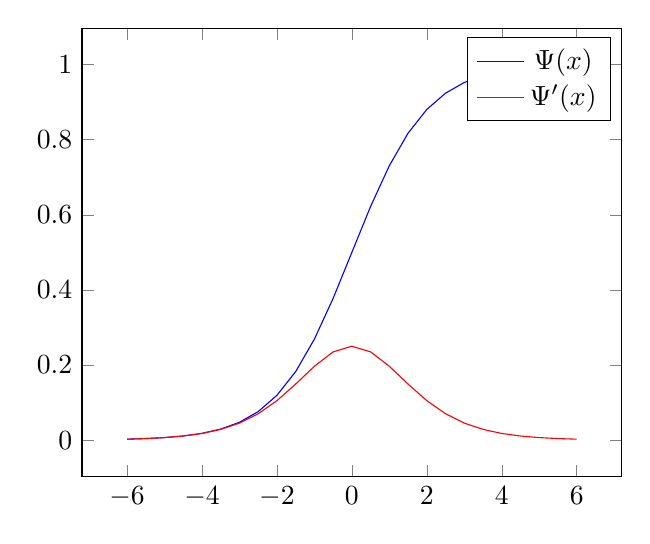
\begin{tikzpicture}
            \begin{axis}[]
                \addplot[domain = -6:6,blue] {1/(1+exp(-x))};
                \addplot[domain = -6:6,red] {(exp(-x))/(1+exp(-x))^2};
                \legend{
                    $\Psi(x)$,
                    $\Psi^{\prime}(x)$
                }
            \end{axis}
        \end{tikzpicture}
        \caption{Graphen der Sigmoid-Aktivierungsfunktion $\Psi(x)=\frac{1}{1+e^{-x}}$ und dessen Ableitung.}
        \label{sigmoid-figure}
    \end{center}
\end{figure}
Sobald $|x|$ groß wird, ist die Ableitung $\Psi'(x) \approx 0$ (siehe Abbildung \ref{sigmoid-figure}). Dies hat die Auswirkung, dass
$\delta_j^{(L)}$ bei betragsmäßig großen Signalen um den Faktor $\Psi'(s_j^{(L)})$ kleiner wird. Dadurch werden die
nachfolgenden Werte
\[
    \delta_i^{(l-1)}=\Psi'(s_i^{(l-1)})\sum\limits_{j=1}^{n^{(l)}}\delta_j^{(l)} \omega_{ij}^{(l)}
\]
auch immer kleiner, da sowohl $\delta_j^{(l)}$ als auch $\omega_{ij}^{(l)}$ klein sind. Die Werte von $\delta_i^{(l)}$ werden
so klein, dass sie gewichtet mit hinreichend kleiner Lernrate ($\eta <1$) im Gradientenverfahren keine Auswirkung
auf das neue Gewicht haben. Für ein allgemeines Gradientenverfahren gilt dann
\[
    \omega_{ij}^{(l)[k+1]} = \omega_{ij}^{(l)[k]}\underbrace{-\eta \delta_j^{(l)[k]}x_i^{(l-1)[k]}}_{\approx 0}\approx \omega_{ij}^{(l)[k]}.
\]
Um diesem Problem entgegenzuwirken, gibt es mehrere Verbesserungsmöglichkeiten.\newline
$\textbf{Möglichkeit 1}:$ Man wählt eine andere Aktivierungsfunktion. Die Effektivität des allgemeinen
Gradientenverfahren sinkt rapide bei Funktionen mit Plateaus. Da die Sigmoidfunktion bei betragsmäßig großen Signalen
für einen verschwindenden Gradienten $\nabla C$ sorgt (was zu Plateaus führt), ist sie für neuronale Netze mit mehreren
versteckten Schichten nicht geeignet. Aktivierungsfunktionen, wie zum Beispiel die ReLU-Funktion $\Psi(x)=\max(0,x)$ mit
der Ableitung $\Psi'(x)= \begin {cases} 0, &\text{x}\leq 0\\ 1, &\text{x}>0\end{cases}$, sind besser geeignet für tiefe neuronale
Netze, da dessen Ableitungen keine verkleinernde Wirkung auf $\delta_i$ haben, sodass der Gradient $\nabla C$ nicht
verschwindet.\\
$\textbf{Möglichkeit 2}:$ Eine geschicktere Initialisierung der Gewichte $\omega_{ij}^{(l)}$ wie in Abschnitt
\ref{subsec:gewichtsinitialisierung}\\
$b)$ $\textbf{explodierender Gradient}:$
Analog zum verschwindenden Gradienten existiert auch das Problem des \textit{explodierenden} Gradienten, in dem
$\delta_j^{(l)}>1$ ist.\\
Angenommen: Die Gewichte sind zufällig initialisiert, wobei für alle $\omega_{ij}^{(l)}>1$ und $b_j^{(l)}=0$
gilt. Bei linearer Regression werden die Signale $s_j^{(l)}$  beispielsweise für wachsendes $l$ immer größer, da

\[
    x_j^{(l)}=\Psi(s_j^{(l)})=\Psi\left( \sum\limits_{i=1}^{n^{(l)}} \underbrace{\omega_{ij}^{(l)}x_{i}^{(l-1)}}_{>1} \right)
\]
gilt. Solange $\frac{\partial C}{\partial y_i} > 1$ gilt bei einer Aktivierungsfunktion mit $\Psi'(x)>1$ auch $\delta_j^{(L)}>1$,
was zu einem explodierenden Gradienten $\nabla C$ führt. Falls $\Psi'(x)=1$ (wie beispielsweise für die ReLU-Funktion bei
positiver Eingabe oder linearer Aktivierungsfunktion), so werden die Werte der $\delta_i^{(l)}$ zwar nicht direkt von der Ableitung
der Aktivierungsfunktion beeinflusst, aber bei einem sehr tiefgehendem Netz ($L>50$) werden die Werte der $\delta_i$ trotzdem
groß, da $\omega_{ij}^{(l)}>1$ gilt. Ähnlich wie beim verschwindenden Gradienten werden wir später eine geschickte
Initialisierung der Gewichte herleiten, um diesem Problem entgegenzuwirken.

\subsubsection{Batch Training}
Während des Lernprozesses eines neuronalen Netzes wird über die gesamten Eingangsdaten $X^{(0)}$ iteriert. Dabei nennt
man ein einzelnes Element von $X^{(0)}$ \textit{Probe} (engl. sample). Eine Ansammlung an Proben heißt wiederum
\textit{Batch}. Außerdem werden die Lernprozesse auch \textit{Epochen} genannt, dessen Anzahl angibt, wie oft das
neuronale Netz die gegebenen Eingangsdaten zum Training nutzt. Es macht Sinn, die Eingangsdaten in Batches einzuteilen,
denn so wird Speicherplatz gespart und an Rechengeschwindigkeit gewonnen, da die Gewichte erst nach dem Durchgang eines
Batches aktualisiert werden, anstatt sie nach jeder Probe zu berechnen. Dies wird realisiert, indem wir die Gradienten
der Proben in einem Batch mit Hilfe der Backpropagation berechnen und im Anschluss den Durchschnitt
\[
    \widetilde{\nabla C} = \frac{1}{|B|} \sum_{i=1}^{|B|} \nabla C(X^{(0,i)})
\]
verwendet, wobei $|B|$ die Größe der Batches angibt und $X^{(0,i)}$, $1 \leq i \leq |B|$, eine Probe des Batches $B$ ist.
Dieser Mittelwert wird dann durch das gegebene Gradientenverfahren verwendet, um die Gewichte $\omega_{ij}^{(l)}$ zu
aktualisieren. Dabei spielt die Größe der Batches $|B|$ eine wichtige Rolle, denn wenn $|B|$ zu klein ist, so werden die
Abschätzungen des Durchschnitts zu ungenau, was wiederum den Lernprozess verlangsamen würde. Da wir jeden Batch jedoch
nur einmalig verwenden und anschließend neue zufällige Trainingsdaten erstellen, werden wir die Gesamtanzahl der
Batches mit Epochen identifizieren. Also ist jeder Batch eine Epoche.

\subsection{Prinzip der Lösungspakete}
\label{subsec:lsgpakete}
Wir werden uns in diesem Abschnitt an der wissenschaftliche Arbeit \cite{flamantSolvingDifferentialEquations2020}
orientieren. Unsere Problemstellung liefert im Allgemeinen keine beschriebene Datenmenge (engl. labeled data), mit der
wir unser neuronales Netz trainieren können. Wir haben lediglich die gewöhnliche Differentialgleichung erster Ordnung
\begin{align}
    \label{dgl-machinelearnung}
    x^{\prime} = f(t,x)
\end{align}
mit den Anfangsbedingungen $x(t_0)=x_0$ gegeben. Dabei definieren wir die Funktion
\begin{align}
    \label{g-func}
    &G:\mathbb{R}^n \times \mathbb{R}^n \times [t_0, t_f] \times \mathbb{R}^p \rightarrow \mathbb{R}^n \nonumber\\
    &G \left( x, x^{\prime}, t, \theta \right) = x^{\prime} - f(t, x, \theta),
\end{align}
wobei $p$ die Anzahl der physikalischen Parametern ist. Hierfür werden wir ein sogenanntes \textit{Lösungspaket}
(engl. solution bundle) bilden, welches aus den Lösungen der Gleichung \eqref{g-func} besteht.
\begin{definition}
    \label{sol-bundle}
    Seien die Teilmengen $X_0 \subset \mathbb{R}^n$, $\Theta \subset \mathbb{R}^p$ und $[t_0,t_f] \subset \mathbb{R}$
    gegeben. Dann heißt
    \[
        x(t;x_0, \theta)
    \]
    Lösungspaket der gewöhnlichen Differentialgleichung \eqref{g-func}, wobei $t \in [t_0,t_f]$, $x_0 \in X_0$ und
    $\theta \in \Theta$.
\end{definition}
Unser Ziel ist es diese Lösungspakete mit Hilfe neuronaler Netze zu approximieren. Wir definieren die Approximation der
Lösung über $(X_0,\Theta)$ mit
\begin{align}
    \label{nn-approx}
    \hat{x}(t;x_0, \theta) = x_0 + a(t) N(t; x_0, \theta; \omega),
\end{align}
wobei $N:\mathbb{R}^{1+n+p} \rightarrow \mathbb{R}^n$ das neuronale Netz mit den Gewichten $\omega$ repräsentiert und
$a:[t_0,t_f] \rightarrow \mathbb{R}$ hat die Eigenschaft $a(t_0)=0$. Hierdurch wird das Erfüllen der
Anfangswertbedingungen in der Approximation \eqref{nn-approx} sichergestellt. Durch Tests in
\cite{flamantSolvingDifferentialEquations2020} wurde herausgefunden, dass $a$ der Form
\[
    a(t) = 1 - e^{t_0-t}
\]
besonders gut geeignet ist. Zusammengefasst wollen wir für jedes Lösungspaket $(t_i,x_{0i}, \theta_i)$ eine Approximation
$\hat{x}$ finden, so dass
\[
    G(\hat{x}(t_i;x_{0i},\theta_i), \hat{x}^{\prime}(t_i;x_{0i},\theta_i),t_i,\theta_i) \approx 0.
\]
Die Kostenfunktion ergibt sich dann durch
\begin{align}
    \label{cost-func}
    \mathcal{C} = \frac{1}{|B|} \sum_{(t_i,x_{0i},\theta_i) \in B} \mu(t_i)
    \left\lVert G(\hat{x}(t_i;x_{0i},\theta_i), \hat{x}^{\prime}(t_i;x_{0i},\theta_i),t_i,\theta_i) \right\rVert_2^2,
\end{align}
wobei $\mu:[t_0,t_f] \rightarrow \mathbb{R}$ durch $b(t) = e^{\lambda (t_0 - t)}$ gegeben ist. Die Batches \textit{B}
bestehen aus Ansammlungen von 3-Tupel $(t_i,x_{0i},\theta_i)$, also
$B=\{(t_i,x_{0i},\theta_i) \in [t_0,t_f] \times X_0 \times \Theta\}$ mit der Kardinalität $|B|$, welche batch size genannt wird. Mit
vorgegebenen Gebieten für $X_0$ und $\Theta$ durch die Problemstellung (bspw. physikalische Zusammenhänge der gegebenen
Differentialgleichung) können die Eingabewerte bestimmt werden. Dafür genügt in den meisten Fällen eine zufällige
Wahl aus einer Gleichverteilung der Mengen $X_0$ und $\Theta$. Da wir in unserer Anwendung theoretisch unendlich
Eingangsdaten zur Verfügung haben, kann der Begriff einer \textit{Epoche} nicht definiert werden. Stattdessen
repräsentiert jeder Batch eine einzigartige Probe die für den Trainingsablauf genutzt wird, wobei eine steigende
Anzahl der Proben eine bessere Approximation liefert. Das Problem des \textit{Overfittings} kann hierbei nicht
auftreten, da es nicht zu viele relevante Variablen bzw. Trainingsdaten gibt. Der Korrekturfaktor $\mu(t_i)$ wird zur
Beeinflussung des lokalen Fehlers
\begin{align*}
    \tau(t_i;x_{0i}, \theta_i)
    := G \left( \hat{x}(t_i;x_{0i}, \theta_i), \hat{x}^{\prime}(t_i;x_{0i}, \theta_i),t_i;\theta_i \right)
\end{align*}
eingeführt. Ähnlich wie in Satz \ref{one-step-error-bound} für Einschrittverfahren können wir auch hier einen
Zusammenhang des lokalen und des globalen Fehlers des neuronalen Netzes zeigen. Dabei ist der globale Fehler des
neuronalen Netzes gegeben mit $e(t) = \hat{x}(t) - x(t)$, wobei $x$ die Lösung von \eqref{dgl-machinelearnung} ist.
\begin{satz}
    \label{ml-error}
    Für \eqref{dgl-machinelearnung} ist der lokale Fehler $\tau$ gegeben durch
    $\tau(t) = \hat{x}^{\prime}(t) - f(t,\hat{x})$. Es gilt
    \[
        \left\lVert e(t) \right\rVert_2 = \frac{\tau_{t_f}}{L} \left( e^{L(t-t_0) - 1} \right),
    \]
    wobei $\tau_{t_f} = \max\limits_{t_0 \leq t \leq t_f} \left\lVert \tau(t) \right\rVert_2$ und $L$ die
    Lipschitz-Konstante der rechten Seite $f$.
\end{satz}
$Beweis.$ Der lokale Fehler ergibt sich durch einfaches Konstuierens von $G$.\\
Für den globalen Fehler $e(t) = \hat{x}(t) - x(t)$ gilt
\begin{align*}
    \hat{x}(t) = e(t) + x(t).
\end{align*}
Einsetzen in den lokalen Fehler ergibt
\begin{alignat*}{2}
    &\tau(t) &= e^{\prime}(t) + x^{\prime}(t) - f(t,e(t)+x(t))\\
    \text{oder} \quad &e^{\prime}(t) &= \tau(t) - x^{\prime}(t) + f(t,e(t) + x(t)),
\end{alignat*}
wobei $x$ die Lösung von \eqref{dgl-machinelearnung} ist , also $x^{\prime}=f(t,x(t))$. Des Weiteren ist $f$
Lipschitz-stetig im zweiten Argument,
das heißt es gilt $\left\lVert f(t,x(t)+e(t)) - f(t,x(t)) \right\rVert_2 \leq L \left\lVert e(t) \right\rVert_2$. Also kann
man die Norm der rechten Seite obiger Gleichung schreiben als
\begin{align*}
    \left\lVert \tau(t) + f(t,e(t) + x(t)) - x^{\prime}(t) \right\rVert_2
    &= \left\lVert \tau(t) + f(t,e(t) + x(t)) - f(t,x(t)) \right\rVert_2 \\
    &\leq \left\lVert \tau(t) \right\rVert_2 + L\left\lVert e(t) \right\rVert_2 \\
    &\leq \tau_{t_f} + L \left\lVert e(t) \right\rVert_2.
\end{align*}
Dabei wurde die Dreiecksungleichung benutzt und der lokale Fehler wurde durch das Maximum aller lokalen Fehler
abgeschätzt. Jetzt suchen wir eine Funktion $E(t)$ die folgende Gleichung erfüllt
\[
    E^{\prime}(t) = \tau_{t_f} + L E(t),
\]
wobei $0 \leq \left\lVert e(t) \right\rVert_2 \leq E(t)$ und $E(t_0) = 0$ gilt. Also haben wir eine lineare gewöhnliche
Differentialgleichung erster Ordnung, dessen Lösung sich mit \eqref{linear-ode-solution} berechnen lässt
\begin{align*}
    E(t) &= e^{L(t-t_0)}E(t_0) + \int_{t_0}^{t}e^{L(t-s)}\tau_{t_f} ds \\
    &= \tau_{t_f} e^{Lt} \int_{t_0}^{t}e^{-Ls} ds \\
    &= \frac{\tau_{t_f} }{L} \left( e^{L(t-t_0)} - 1 \right).
\end{align*}
Daraus folgt
\[
    \left\lVert e(t) \right\rVert_2 \leq \frac{\tau_{t_f}}{L} \left( e^{L(t-t_0)} - 1 \right),
\]
was sich mit der Abschätzung in Satz \eqref{one-step-error-bound} vergleichen lässt. \qedwhite\\
Hierdurch erkennt man, dass der globale Fehler durch einen frühen lokalen Fehler exponentiell mit der Zeit wachsen
kann. Deshalb ist es sinnvoll, die exponentiell fallende Korrekturfunktion $b$ zu nutzen, um den lokalen Fehler in
frühen Zeitpunkten zu skalieren.

\subsection{Intervall-Lernen}
\label{subsec:curriculum-learning}
Beim Approximieren von gewöhnlichen Differentialgleichungen mithilfe von Lösungspaketen ist es unser Ziel, die
Kostenfunktion so gut wie möglich zu minimieren. Dabei kann ein Fehler am Anfang des Trainingsprozesses schon dazu
führen, dass das neuronale Netz das gegebene Anfangswertproblem nicht approximiert, wie in Satz \ref{ml-error} zu sehen
ist. Genauer wird die Trajektorie der approximierten Funktion durch den Fehler in andere Bereiche des Phasenraums
geleitet. Dies wiederum sorgt für einen größeren globalen Fehler, da nun ein anderes Anfangswertproblem approximiert
wird. Eine mögliche Behebung dieses Problems ist das Prinzip des sogenannten \textit{Intervall}-\textit{Lernens}
(eng. curriculum learning). Eine allgemeine Diskussion dieses Prinzips lässt sich in \cite{bengioCurriculumLearning2009}
nachlesen. Für das Approximieren von gewöhnlichen Differentialgleichungen nutzen wir das Intervall-Lernen so, dass wir
das Intervall der Zeiten $[t_0, t_f]$ begrenzen. Hierzu werden wir die Batches $B$ bearbeiten, also erhalten wir neue
Batches $B^{\prime}$ mit
\[
    B^{\prime}:=  \{(t_i,x_{0i},\theta_i) \in [t_0,t_m] \times X_0 \times \Theta\},
\]
wobei $t_m<t_f$ und $m$ die Anzahl der bereits trainieren Batches ist. Wir lassen also das neuronale Netz zuerst mit
einer kleinen Menge an Daten trainieren, um problematische Stellen, die zu einer Verschiebung der Trajektorien sorgen,
zu vermeiden. Dabei wird ie Menge der Daten in Abhängigkeit der bereits trainierten Batches erhöht. In Kapitel
\ref{sec:verfahrensvergleich} werden wir
\[
    t_m = \frac{t_f}{\ln(11)} \ln(10 \frac{m}{|B|} + 1), \qquad m = 1, \dots, |B|,
\]
zur Beschränkung des Zeitintervalls verwenden.

\subsection{Gewichtsinitialisierung}
\label{subsec:gewichtsinitialisierung}
Die Gewichtsinitialisierung ist ein entscheidender Faktor um Probleme des explodierenden und verschwindenden Gradienten
entgegenzuwirken. In diesem Abschnitt werden wir ein Intervall bestimmen, welches dann zur Initialisierung der Gewichte
$\omega_{ij}$ genutzt wird. Dazu werden wir die $(l-1)$-te und $l$-te Schicht eines neuronalen Netzes und die
zugehörigen Gewichte $\omega_{ij}:=\omega_{ij}^{(l)}$ sowie $x_{i}^{(l-1)}$ als unabhängige, identisch verteilte
Zufallszahlen betrachten. Außerdem gilt für den Erwartungswert der Gewichte $\mathbb{E}(\omega_{ij})=0$ und die bias $b$
werden mit $0$ initialisiert. Genaueres zur Berechnung folgender Varianzen lässt sich in
\cite[191-195]{ovidiucalinDeepLearningArchitectures} nachlesen. Für die Varianz der Ausgabe der $l$-ten Schicht
$x_i^{(l)}$ ergibt sich
\begin{align*}
    Var(x_j^{(l)}) = n^{(l-1)} \Psi^{\prime}(0)^2 Var(\omega_{ij}) Var(x_i^{(l-1)}).
\end{align*}
Unter der Voraussetzung, dass die Varianz der beiden Schichten gleich bleibt, also \\
$Var(x_j^{(l)})=Var(x_j^{(l-1)})$, so ergibt sich für die Varianz der Gewichte
\[
    Var(\omega_{ij}) = \frac{1}{n^{(l-1)}\Psi^{\prime}(0)^2}.
\]
Die gegebene Voraussetzung macht Sinn um die oben erwähnten Probleme des explodierenden bzw. verschwindenden Gradienten
zu vermeiden. Genau wie bei der Varianz der Ausgaben $x_j^{(l-1)}$ und $x_j^{(l)}$ ist es auch vorteilhaft die Varianz
der Kostenfunktion ausgehend von der Backpropagation gleichzustellen. Also folgt aus
\[
    Var(\frac{\partial C}{\partial \omega_{ij}^{(l-1)}}) = Var(\frac{\partial C}{\partial \omega_{ij}^{(l)}})
\]
mit Hilfe einiger stochastischer Umformungen und der Annahme, dass $\Psi(x)=x$, die Gleichung
\[
    Var(\delta_j^{(l-1)}) = Var(\delta_j^{(l)}),
\]
wobei $\delta_j^{(l)}$ eine aus der Backpropagation resultierende Variable ist. Hiermit folgt für Varianz der Gewichte
\[
    Var(\omega_{ij}) = \frac{1}{n^{(l)}}.
\]
Das Erfüllen beider Voraussetzungen führt zu einer restriktiven Bedingung $n^{(l-1)} = n^{(l)}$, weshalb man sich für
\[
    Var(\omega_{ij})= \frac{2}{n^{(l-1)} + n^{(l)}}
\]
einigt. Werden die Gewichte nun gleichverteilt auf $[-a,a]$, dessen Varianz $\frac{a^2}{3}$ gleichgestellt mit der
Varianz der Gewichte $a=\frac{\sqrt {6}}{\sqrt {n^{(l-1)} + n^{(l)}}}$ ergibt, also
\[
    \omega_{ij} \sim
    \left[ -\frac{\sqrt {6}}{\sqrt {n^{(l-1)} + n^{(l)}}}, \frac{\sqrt {6}}{\sqrt {n^{(l-1)} + n^{(l)}}} \right]
\]
für alle $i = 1, \dots, n^{(l-1)}$, $j=1,\dots,n^{l}$, $l=1,\dots,L$ Diese Verteilung heißt \textit{Xavier-} oder
\textit{Glorot-Initialisierung}. In Betracht der Aktivierungsfunktion $\Psi(x)=\tanh(x)$ kann eine Initialisierung mit d
er Gleichverteilung
\[
    \omega_{ij} \sim
    \left[ -\frac{\sqrt {6}}{\sqrt {n^{(l-1)} \tanh(2)}}, \frac{\sqrt {6}}{\sqrt {n^{(l-1)} \tanh(2)}} \right]
\]
gefunden werden (vgl. hierbei \cite[27]{remcovandermeerSolvingPartialDifferential}).

%\subsection{Fortsetzen einer Wahrscheinlichkeitverteilung}
%\label{subsec:fortsetzeneinerwahrscheinlichkeitsverteilung}
%Es ist möglich eine Wahrscheinlichkeitsverteilung der Anfangsbedingungen diese mit Hilfe sowohl eines
%Runge-Kutta-Verfahrens als auch neuronalen Netzen fortzusetzen. Der Vorteil hierbei ist es beispielsweise bei der
%die Wahrscheinlichkeit der Position eines Körpers im Weltall zu einem bestimmten Zeitpunkt $t$ berechnen zu können. Für
%Details zur Nutzung von (impliziten) Runge-Kutta-Verfahren wird auf \cite{aristoffIMPLICITRUNGEKUTTAMETHODS} verwiesen.
%Obwohl Runge-Kutta-Verfahren sehr genau sind, haben neuronale Netze den Vorteil, eine Funktion simulieren zu können.
%Es muss also für die gefragte Zeit $t$ nicht iteriert werden, sondern kann einfach eingesetzt werden. Außerdem können
%so für mehrere verschiedene physikalische Parameter Wahrscheinlichkeitsverteilungen angegeben werden, ohne jede
%Approximation einzeln berechnen zu müssen. Sei also ein trainiertes neuronales Netz gegeben. Das Lösungspaket
%$x(t; x_0)$ gibt eine Koordinatentransformation von $x_0$ nach $x_t$ an. Unter der Annahme, dass die Transformation
%$f: X_0 \rightarrow X_t, f(x_0) = x(t;x_0)$ invertierbar und differenzierbar ist, kann die Wahrscheinlichkeitsverteilung
%eines späteren Zeitpunktes $t$ angegeben werden mit
%\[
%    p_t(x_t) = p_0(f^{-1}(x_t)) \left\lVert J_{f^{-1}} \right\rVert_2,
%\]
%wobei $f^{-1}(x_t)$ das Inverse der Transformation $f(x_0)=x(t;x_0)$ und $J_{f^{-1}}= \frac{\partial x_0}{\partial x_t}$
%die Jacobi-Matrix von $f^{-1}$ ist. Falls jedoch die Wahrscheinlichkeitsverteilung der Anfangszeit $p_0(x_0)$ gesucht
%ist, so lässt sich diese ohne Inverse berechnen lassen:
%\[
%    p_0(x_0) = p_t(f(x_0))\left\lVert J_f \right\rVert_2,
%\]
%wobei $J_f= \frac{\partial x_t}{\partial x_0}$ die Jacobi-Matrix von $f$ ist. Da das Generieren einer Zufallszahl aus
%der Wahrscheinlichkeitsverteilung $p$ in der Regel mit hohem Rechenaufwand verbunden ist, nutzt man bei zu großen
%Dimensionen der Anfangsbedingungen und physikalischen Parametern stattdessen sogenannte
%\textit{Markow-Ketten-Monte-Carlo-Verfahren} (kurz MCMC-Verfahren). Diese wählen die gesuchten Daten mit Hilfe einer
%Markow-Kette und sind Dimensionsunabhängig: Genaueres zu MCMC-Verfahren kann in \cite{SamplingMethods} nachgelesen
%werden.
